\documentclass[12pt]{article}
\usepackage[a4paper, total={18cm, 25cm}, left=1.5cm, top=2.5cm]{geometry}
\usepackage[english]{babel}
\usepackage[utf8]{inputenc}
\usepackage{csquotes}
\usepackage[unicode]{hyperref}
\usepackage[T1]{fontenc}
\usepackage{xcolor}
\usepackage{setspace}
\usepackage{graphicx}
\usepackage{listings}
\usepackage{amsmath}

\lstset{
  basicstyle=\itshape,
  xleftmargin=3em,
  literate={->}{$\rightarrow$}{2}
           {α}{$\alpha$}{1}
           {δ}{$\delta$}{1}
}

\title{VYPa compiler construction documentation}
\author{Authors: xmudry01, xpauld00}
\date{December 2022}

\begin{document}
\null  % Empty line
\nointerlineskip  % No skip for prev line
\begin{center}
    
\includegraphics[scale=0.1]{images/fit_logo.png}
\end{center}
\vfill
\let\snewpage \newpage
\let\newpage \relax
\maketitle
\begin{center}
Point division: 50/50\\
Implemented extensions: MINUS    
\end{center}
\let \newpage \snewpage
\vfill 
\break % page break

\section{Technologies and tools}

We chose to use Python as our programming language with version 3.8+, because of it has good abstraction capabilities and standard library. We also decided to use PLY (Python Lex-Yacc) library for our lexer and parser.

\subsection{Installation and setup}

Firstly, the program has to be run with \emph{make} (which runs the \emph{make init} command) to install and configure all dependencies. Then you can run the compiler with:
\\
\begin{lstlisting}[language=bash,basicstyle=\ttfamily\normalsize\bfseries]
./vypcomp INPUT_FILE [OUTPUT_FILE]
\end{lstlisting}


\section{Grammar}
We have defined following grammar (figure \ref{fig:grammar}) with non-terminals being represented by lowercase words and terminals with uppercase words. 

\subsection{Lexical analysis}
Lexical analysis has been implemented with PLY library lexer. We simply create tokens based on regular expressions which are being matched with the input source code. If the input is correct, tokens are passed passed to the parse. Otherwise the program exits and returns error code 11. 

\subsection{Syntax analysis}
Syntax analysis has been implemented with PLY library yacc parser.
Parser accepts tokens created in lexer and performs syntax analysis.
If the input is correct, the output is a tuple of tuples which represents our parse tree. Otherwise the program exits and returns exit code 12.

Afterwards we use our custom Python classes for abstracting \emph{functions} (containing function name, return type, parameters and function body), \emph{classes} (containing class name, superclass, properties and functions) and \emph{variables} (containing variable type and name) to make them easier to work with.

\begin{figure}
\begin{lstlisting}[mathescape]
start -> program
program -> func_def program | class_def program | $\varepsilon$
func_header -> var_type ID LPAREN param_list RPAREN
func_body -> statement_new_scope
param_list -> VOID | func_param
func_param -> func_param_def next_param
func_param_def -> var_type ID
next_param -> , func_param | $\varepsilon$
class_def -> CLASS ID , ID class_body
class_body -> LBRACE class_member_list RBRACE
class_member_list -> class_member | $\varepsilon$
class_member -> class_member_def class_next_member
class_member_def -> var_def | func_def
class_next_member -> class_member | $\varepsilon$
var_type -> INT | STRING | ID
statement -> var_def statement | var_assignment statement 
| statement_expr statement | statement_return statement | 
statement_while statement | statement_if statement | 
statement_this statement | statement_id statement | $\varepsilon$
statement_new_scope -> LBRACE statement RBRACE statement_scope_end
statement_scope_end -> $\varepsilon$
statement_if -> IF LPAREN expr RPAREN statement_new_scope
ELSE statement_new_scope
statement_while -> WHILE LPAREN expr RPAREN statement_new_scope
stetement_return -> RETURN expr SEMI | RETURN SEMI
statement_this -> THIS PERIOD ID EQUALS expr SEMI 
| SUPER PERIOD ID EQUALS expr SEMI
statement_id -> ID PERIOD ID EQUALS expr SEMI
statement_expr -> expr SEMI
var_assignment -> ID EQUALS expr SEMI
var_def -> var_type ID multiple_var_def
multiple_var_def -> SEMI | COMMA ID multiple_var_def
expr -> LPAREN expr RPAREN
expr -> INT_CONST | STRING_CONST | ID
expr -> MINUS expr | PLUS expr
expr -> expr PLUS expr | expr MINUS expr | expr TIMES expr 
| expr DIVIDE expr
expr -> LNOT expr
expr -> expr LOR expr | expr LAND expr
expr -> expr LT expr | expr LE expr | expr GE expr | expr GT expr 
| expr EQ expr | expr NE expr
expr -> LPAREN INT RPAREN expr | LPAREN STRING RPAREN expr
expr -> NEW ID
expr -> ID PERIOD expr | THIS PERIOD expr | SUPER PERIOD expr
expr -> ID LPAREN expr_list RPAREN | ID LPAREN RPAREN
expr_list -> expr next_expr
next_expr -> COMMA expr next_expr | $\varepsilon$
\end{lstlisting}
\caption{Grammar definition}
\label{fig:grammar}
\end{figure}

\newpage
\section{Abstract syntax tree}
To easily generate body of functions VYPcode we converted their derivation tree to an abstract syntax tree.
It is being created with a Node class, which has \emph{name}, \emph{type}, \emph{value}, \emph{left and right child}.

\begin{figure}[ht]
    \centering
    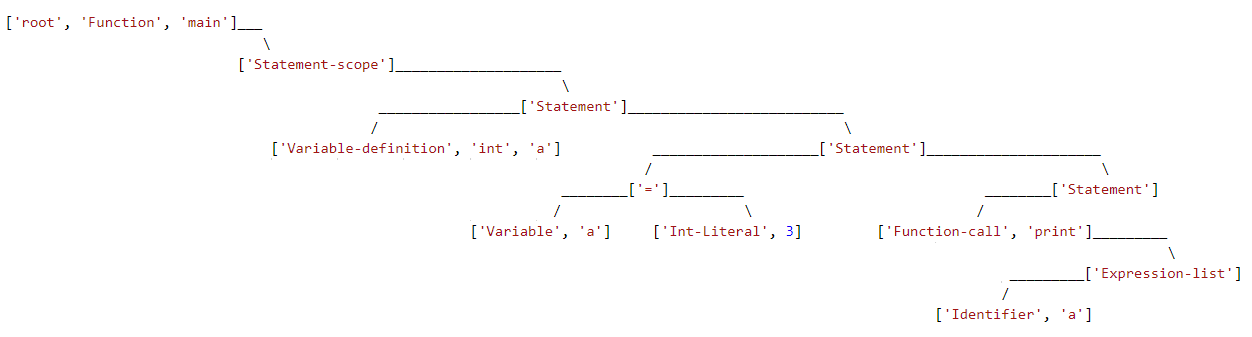
\includegraphics[scale=0.8]{images/ast.png}
    \caption{Example abstract syntax tree}
    \label{fig:ast}
\end{figure}

\section{Semantic analysis}
Semantic analysis is being done by passing through abstract syntax tree and checking assign, function call, return, etc. nodes. Afterwards we search functions and variables in the symbol table and compare their declared types with assign value, number of parameters and types in a function, return type of the function with value being returned. Symbol table is keeping track of functions and variables in respective scopes. It is being represented by list of dictionaries, where first dictionary contains all classes and functions and other dictionaries contain function scope and code block scopes.

\section{Code generation}
We chose direct code generation from the AST instead of implementing any optimizations as it is the fastest approach to compile code. For code generation we implemented class \emph{CodeGenerator} which was responsible for the output and traversing abstract syntax trees to generate code. During the traversal each node in AST is checked and the resulting VYPcode is appended to the output according to the subtree structure. To easily create output we implemented class \emph{CodeTemplate} which takes care of the subtree output generation. To easily create VYPcode we implemented \emph{Instruction} class which returns instructions with provided parameters.\\

We used registers as follows:
\begin{itemize}
  \item \$0 - Function pointer which points to the stack
  \item \$1 - PC restore register
  \item \$2 - Return value register
  \item \$3 - First Expression Result
  \item \$4 - Second Expression Result
  \item \$5 - Chunk pointer
  \item \$6 - First miscellaneous register
  \item \$7 - Second miscellaneous register
\end{itemize}

\subsection{Variables}
Variables are are added to the symbol table corresponding to the current scope on AST traversal.
Register \$0 is used to point to variables on the stack, relative to the function pointer's value, which points to the start of a scope on the stack. Index of the variable is used as offset from the function pointer's position and is being calculated by its position of the variable in the symbol table. 

\subsection{Function calls}
Before a function call, parameters of the function and the current position of the function pointer register are pushed on the stack. Afterwards when a function is called the program counter is pushed to stack, function pointer is set to point at the new top of the stack and variables representing parameters of the function are created. After the function is executed, the stack is shifted backwards by the number of pushed parameters, function pointer is set back to the previous function scope and resulted value is stored in register \$2 and the stored program counter value is returned, exiting the function and jumping back to the line of code where the function was called from, continuing the execution.

\subsubsection{Embedded functions}
Short embedded function which result in short sequence of instructions such as \emph{readInt} and \emph{readString} are not implemented via assembly function calls, because the number of instruction needed to prepare the function call and clean up the stack after is higher than just repetitively using the few same instructions.

Longer embedded functions like \emph{length}, \emph{subStr}, \emph{concat} (used on string concatenation with \textbf{+} operator) and user-defined functions are implemented via proper assembly function calls.

\subsection{Expressions}
Expressions are on AST represented by \emph{Function-call}, \emph{Expression-list}, \emph{Next-expression}, \emph{Unary} (expression) and \emph{Binary} (expression) nodes. Left child node always has a concrete value or is an identifier, whereas the right child node can also be a next expression node, chaining expressions with more than 2 operands.

Expressions operators precedence is defined in a table stored in the parser. 
At first expressions are stored in derivation tree in the pre-order notation. Afterwards the expressions are being represented in abstract syntax tree such, that they can be generated by post-order traversal. 

Expressions are executed by pushing operands to the stack and using respective operations with the result of the expression saved either to register \$3 or \$4.

\subsection{Classes}

Not implemented.

\newpage
\section{Work division}
We worked together on syntax analysis, code generation from abstract syntax tree and conversion from derivation tree to abstract syntax tree,
Adam Múdry (xmudry01) was responsible for lexical analysis, abstraction of code generation, test suite and setup of the project.
Daniel Paul (xpauld00) was responsible for abstraction of functions, variables and classes, semantic checks and handling of derivation tree.
For this reason we split the evaluation result 50/50.

\section{References}
Ply (python lex-yacc). PLY (Python Lex-Yacc) - ply 4.0 documentation. (n.d.). Retrieved November 12, 2022, from https://ply.readthedocs.io/en/latest/ply.html 
\end{document}
